\documentclass[letterpaper,12pt]{article}

% --- PAQUETES DE IDIOMA
\usepackage[spanish,mexico]{babel}
\usepackage[utf8]{inputenc}
\usepackage{csquotes}

% --- PAQUETES MATEMÁTICOS --
\usepackage{amsmath}
\usepackage{amssymb}
\usepackage{cancel}
\usepackage{mathrsfs}

% --- PAQUETES GRÁFICOS Y DE DISEÑO ---
\usepackage{graphicx}
\usepackage{float}
\usepackage{subcaption}
\usepackage{xcolor}
\usepackage{makecell}
\usepackage{array}
\usepackage{tikz}
\usetikzlibrary{shapes.geometric, positioning}
\usetikzlibrary{shapes.multipart, positioning, arrows.meta, calc, shadows}


% --- PAQUETES DE CÓDIGO ---
\usepackage{listings}
% Configuración del estilo de listings
% Paleta de colores estilo VSCode
\definecolor{codebg}{rgb}{0.95,0.95,0.95}   % gris claro de fondo
\definecolor{keyword}{rgb}{0.0,0.2,0.6}     % azul oscuro
\definecolor{comment}{rgb}{0.25,0.5,0.35}   % verde
\definecolor{string}{rgb}{0.6,0.0,0.0}      % rojo oscuro
\definecolor{number}{rgb}{0.5,0.0,0.5}      % morado

% Paleta de colores personalizada
\definecolor{codegray}{rgb}{0.5,0.5,0.5}
\definecolor{codepurple}{rgb}{0.58,0,0.82}
\definecolor{backcolour}{rgb}{0.95,0.95,0.95}

% Configuración del estilo
\lstset{
  backgroundcolor=\color{backcolour},   % Fondo gris claro
  basicstyle=\ttfamily\small,           % Fuente monoespaciada
  keywordstyle=\color{blue}\bfseries,   % Palabras clave en azul y negrita
  stringstyle=\color{codepurple},       % Cadenas en morado
  commentstyle=\color{codegray}\itshape,% Comentarios grises en cursiva
  numbers=left,                         % Números de línea a la izquierda
  numberstyle=\tiny\color{codegray},    % Estilo de los números
  frame=single,                         % Marco alrededor
  rulecolor=\color{black},              % Color del marco
  breaklines=true,                      % Ajuste automático de línea
  tabsize=4,                            % Tabulación de 4 espacios
  showstringspaces=false                % No mostrar espacios raros
}


% --- RUTAS DE IMÁGENES ---
% LaTeX buscará imágenes en estas carpetas automáticamente
\graphicspath{{img/}{portada_img/}} 

% --- DIBUJO DE CIRCUITOS ---
\usepackage{pgf,tikz}
\usetikzlibrary{decorations.pathreplacing, calc, positioning}

% Definimos el color azul similar al de la imagen
\definecolor{armblue}{RGB}{0, 113, 188}

% --- CONFIGURACIÓN DE PÁGINA (GEOMETRÍA) ---
\usepackage[
    left=25mm, 
    right=25mm,
    top=35mm,
    bottom=30mm,
    headheight=77pt, 
    papersize={21.59cm,27.94cm}
]{geometry}

% --- FORMATO DE TEXTO ---
\renewcommand{\baselinestretch}{1.25} % Interlineado 1.25
\usepackage{parskip} % Espacio entre párrafos sin sangría
\usepackage{lipsum}  % Texto de relleno

% --- VARIABLES GLOBALES ---
\newcommand{\materia}{}

% --- ENCABEZADOS Y PIES DE PÁGINA ---
\usepackage{fancyhdr}
\pagestyle{fancy}
\fancyhf{} % Limpia encabezados y pies por defecto

% CONFIGURACIÓN DE LOS ESCUDOS EN EL ENCABEZADO
\fancyhead[L]{
\includegraphics[height=1.5cm]{portada_img/izq.png}} 
\fancyhead[R]{
\includegraphics[height=1.5cm]{portada_img/der.png}} 

\fancyfoot[C]{\thepage} % Número de página al centro abajo
\renewcommand{\headrulewidth}{0.4pt} % Línea horizontal bajo el encabezado
\renewcommand{\footrulewidth}{0pt}   % Sin línea en el pie

% --- BIBLIOGRAFÍA ---
\usepackage[backend=biber, style=apa, sortcites, url=true]{biblatex}
\addbibresource{referencias.bib}

% --- HIPERVÍNCULOS (Siempre al final del preámbulo) ---
\usepackage{hyperref}
\hypersetup{
    colorlinks=true,
    linkcolor=blue,
    citecolor=blue,
    filecolor=magenta,
    urlcolor=cyan
}

% ---------------------------------------------------------
% INICIO DEL DOCUMENTO
% ---------------------------------------------------------

\begin{document}

    % 1. INSERTAR PORTADA (portada.tex)
    \input{portada.tex}

    \newpage
    \setcounter{page}{1} % Reiniciar contador en 1

    % 2. CONTENIDO
    \noindent\textbf{1.-Explique que son los modos de direccionamiento en la programación de microprocesadores. }

    Los modos de direccionamiento en los microprocesadores es el metodo en el que mediante el cual se calcula la direccion efectiva de los operadores, no obstante para cualquier programador de ensablandor es escencial comprender estos modos de direccionamiento, ya que el direccionamiento no solo define donde esta el dato, sino que tambien cuanto tiempo y energia costara el acceso al mismo.

    Los modos de direccionamiento han ido evolucionando mas entre las arquitecturas CISC y RISC, mientras que las arquitecturas CISC antiguas permitían operaciones aritméticas directamente sobre direcciones de memoria complejas.

    Para esto podemos tener las clasificaciones y sis modos basandose en el ubicacion del operador:

    \begin{enumerate}
        \item Inmediato: El dato es parte de la instrucción.
        \item Registro: El dato está en el banco de registros.
        \item Directo/Absoluto: La dirección de memoria es constante.
        \item Indirecto/Indexado: La dirección se calcula dinámicamente.
    \end{enumerate}

    No obstante, esta clasificacion no es estatica, tenemos el ejemplos de la Raspberry Pi, que es una arquitectura RISC, y a pesar de esto tiene modos de direccionamiento complejos como el modo de direccionamiento indirecto, que es un modo de direccionamiento que se caracteriza por utilizar un registro para almacenar la dirección de memoria del operando, en lugar de incluir la dirección directamente en la instrucción.

    Ahora bien, tenemos el caso de la direccion efectiva, donde es el resultado final de cualuqier calculo de direccion requerido  por una instrucción antes de acceder a la memoria.  La eficiencia con la que una microarquitectura puede calcular esta direccion efectiuva determina el rendimiento en tareas críticas como el recorrido de arreglos, la manipulación de pilas y el acceso a estructuras de datos complejas.

    La implementación hardware de estos modos implica el uso de multiplexores para seleccionar entre diferentes fuentes de datos (el contador de programa, un registro, o un campo de la instrucción) y sumadores para calcular la dirección final.

    \noindent\textbf{2.-Describa el modo de direccionamiento inherente , escriba un ejemplo y un gráfico que represente este modo de direccionamiento.}

    El modo de direccionamiento inherente se conoce tambien como direccionamiento implicito, donde este lo que hace es una representacion mas primitiva y eficiente de instruicciones, en este modo no se especifica expliciamente mediante campos de direccion o seleccion de registros, de hecho es lo opuesto, donde la ubicacion del operando es fija y se asume que el operando esta en un lugar predefinido, como por ejemplo el acumulador o un registro especifico.

    No obstante la instrrciones que modifican el registro de estado, instrucciones de barrera de memoria o tambien las intriccion de NO OPERACION caen en esta categoria conceptual de implicito. Dicho en otras palabras lo anteriormente explicado en el parrafo anterior, lo que hace escencialmente es que el procesador ya entiende implicitamente que no debe alterar ningun estado de los registros, o que debe modificar el estado de los flags, o que no se va a realizar ninguna operacion, lo que hace que este modo de direccionamiento sea muy eficiente en terminos de ciclos de reloj y consumo de energia.

    \textbf{Ejemplo:}

    En el caso de computadoras modernas tenemos el caso de las intrucciones NOP (No Operation), que son instrucciones que no realizan ninguna operación pero que pueden ser útiles para sincronización o para rellenar espacio en el código. En este caso, la instrucción NOP es un ejemplo clásico de direccionamiento inherente, ya que no requiere operandos y su efecto es simplemente no hacer nada.

    Codigo ensablador:
    \begin{lstlisting}[language={[x86masm]Assembler}, caption={Ejemplo de direccionamiento inherente con NOP}]
    NOP ; No Operation, no hace nada
    \end{lstlisting}

    Al decodificar este opcode, la Unidad de Control sabe implícitamente que no debe activar ninguna línea de lectura de memoria ni habilitar la escritura en ningún registro. El "operando" es el propio flujo de tiempo del procesador, consumiendo un ciclo sin efectos secundarios.

    Otro ejemplo en microprocesadores, es la instrucción CLC (Clear Carry). El operando es el bit de acarreo (Carry Flag) en el registro de estado,la instrucción CLC lleva implícita la dirección de ese bit específico..
    
    \textbf{Diagrama:}

    \begin{tikzpicture}[
        node distance=1.5cm,
        font=\small\sffamily,
        % Estilo para la instrucción (Opcode)
        instruction/.style={
            draw=blue!80!black,
            fill=blue!10,
            thick,
            rectangle,
            minimum width=3cm,
            minimum height=1cm,
            rounded corners=3pt,
            drop shadow
        },
        % Estilo para el Registro de Estado (Flags)
        register/.style={
            draw=black,
            fill=white,
            rectangle split,
            rectangle split parts=4,
            rectangle split horizontal,
            minimum height=1cm,
            text width=0.8cm,
            align=center
        },
        % Estilo para la Unidad de Control
        control/.style={
            draw=orange!80!black,
            fill=orange!10,
            trapezium,
            trapezium angle=70,
            minimum width=2.5cm,
            minimum height=1cm,
            thick,
            align=center,
            drop shadow
        },
        % Estilo para etiquetas y flechas
        label/.style={text=gray!40!black, font=\footnotesize\bfseries},
        arrow/.style={->, >=LaTeX, thick, color=gray!80!black}
    ]

        % 1. Nodo: Instrucción (Solo Opcode)
        \node[instruction] (inst) {\textbf{CLC} \\ (Opcode)};
        
        \node[above=0.1cm of inst, label] {Instrucción en Memoria};

        % 2. Nodo: Unidad de Control (Decodificación)
        \node[control, right=2cm of inst] (cu) {Unidad de\\Control};

        % 3. Nodo: Registro de Estado (Target)
        % El Carry Flag es la parte implicita
        \node[register, right=2cm of cu] (flags) {
            \nodepart{one} Z
            \nodepart{two} S
            \nodepart{three} O
            \nodepart{four} \textbf{C}
        };
        
        % Etiquetas para el registro
        \node[above=0.1cm of flags, label] {Registro de Estado (Flags)};
        \node[below=0.4cm of flags, text=red!70!black, font=\scriptsize] (impl) {Ubicación Implícita};

        % Flechas y Conexiones
        
        % Del Opcode a la UC
        \draw[arrow] (inst) -- node[above, font=\scriptsize] {Decodificación} (cu);
        
        % De la UC al Flag específico (Carry)
        % Usamos coordenadas relativas para apuntar exactamente al cuarto compartimento (Carry)
        \draw[arrow, color=red!70!black] (cu.east) -- ++(0.5,0) |- ($(flags.four south) + (0,-0.4)$) -- (flags.four south);

        % Anotación explicativa
        \node[below=1.5cm of cu, align=center, fill=yellow!10, draw=yellow!60!black, rounded corners, inner sep=5pt] (note) {
            \textbf{Direccionamiento Inherente}\\
            El \textit{Opcode} ya indica dónde está el operando.\\
            No hay campo de dirección explícito.
        };

        % Flecha punteada de contexto
        \draw[dashed, gray] (note) -- (cu);

    \end{tikzpicture}

    En la parte izquierda, se observa que la instrucción reside en memoria conteniendo únicamente el Opcode, sin campos adicionales para operandos. Al pasar a la Unidad de Control, esta decodifica la instrucción y sabe implícitamente que debe actuar sobre un recurso específico del procesador: el Flag de Acarreo (C) dentro del Registro de Estado. Como muestra la línea roja, la ubicación del operando destino no se obtiene de una dirección de memoria ni de un índice de registro, lo que resulta en una ejecución rápida y directa.

    \noindent\textbf{3.-Describa el modo de direccionamiento inmediato, escriba un ejemplo y un gráfico que represente este modo de direccionamiento.}

    En este modo de direccionamiento inmediato, el operador fuenteno se queda en una direccion de memoria ni en otro registro, si no que lo que hace es que esta codificado directamente dentro de los bits que conforman la instruccion en si, en otras palabras es que el dato es inmediatamente accesible despues de la busqueda de la instruccion.
    
    La implemetacion de este modo tanto en arquitectura RISC de 32 bits o ARM es dificil de implementar en ambos casos, donde en si el problema principal es en la geometria de la intruccion, por ejemplo si una instruccion tiene una longitud total de 32 bits y debe conener el codigo de operacion, los codigos de condicion y la direccion del registro de destino, es tecnicamente imposible reservar 32 bits adicionales dentro de ella para carar una constante arbitraria de 32 bits.
    Para este problema, se presenta una solucion, donde en arquitecturas ARM, sehace uso del esquema de rotacion, donde en lugar de almacenar la constante tal cual, la instruccion almacena la constante tal cual, la instruccion alamacena un valor base de 8 bits y un valor de rotacion de 4 bits.

    No obstante si se intenta usar una constante que no puede generarse mediante esta rotación (por ejemplo, una constante arbitraria de 32 bits con muchos cambios de bit), el ensamblador generará un error o, si es inteligente, convertirá la instrucción en una carga de memoria (LDR) desde un "literal pool", cambiando efectivamente el modo de direccionamiento de inmediato a relativo al PC, un matiz crítico que Smith advierte a los programadores.

    \textbf{Ejemplo:}

    En el caso de queremos iniciar un contandor en 10, entonces la instruccion en ensamblador seria:
    \begin{verbatim}
        MOV R0, #10
    \end{verbatim}

    Aquí, el símbolo \# (o a veces \$) denota que el 10 es un valor inmediato. El procesador toma el campo de la instrucción correspondiente al operando 2, lo pasa por el "barrel shifter" (desplazador de barril) descrito por Elahi , y deposita el resultado en R0. No se genera ninguna transacción en el bus de memoria de datos. 

    \textbf{Diagrama:}

    \begin{center}
        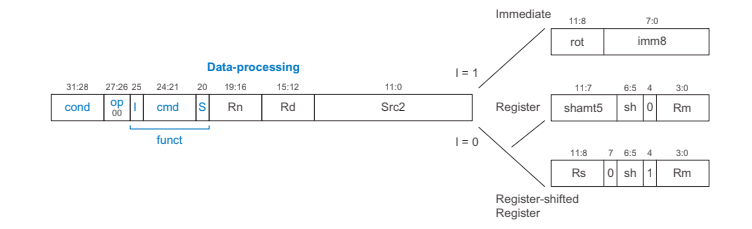
\includegraphics[width=0.8\textwidth]{img/image1.png}
    \end{center}

    Para esto se muestra cómo el operando (dato constante) se encuentra codificado directamente dentro de la propia instrucción, ocupando campos específicos (valor base y rotación) en lugar de residir en una dirección de memoria externa. Este valor es extraído y procesado por el Barrel Shifter para generar la constante final de 32 bits, la cual se deposita inmediatamente en el registro de destino (R0), evitando así cualquier ciclo adicional de lectura en el bus de datos.

    \newpage
    
    \noindent\textbf{4.-Describa el modo de direccionamiento directo, escriba un ejemplo y un gráfico que represente este modo de direccionamiento.}
    
    El modo de direccionamiento diecto tambien es conocido como direccionamiento absoluto, este define el metodo de acceso a memoria en el cual la instruccion. contiene, dentro de sus bits la direccion efectiva que tambein es conocida como EA, este como tal no se requiere ningun calculo complejo, si no que lo que hace la unidad es aue el control del procesador extrae el valor del campo de direccion de la instruccion y ño colocla directamente en el bus de direcciones del sistema para iniciar e¿un ciclo de lectura y escritura.
    
    Para esto el modo de direccionamiento directo ses muy. rapido, donde este sl ya no utilizar la unidsd logica o mejor conocida como ALU para calcular la direccion, no obstante, este modelo sufre de algo conocido como la rigidez, donde si el programa se mueve a otra direccion de memoria entonces las intrucciones tienen que ser reubicadas esto por el caragdor del sistema operativo.

    Cabe recalcar que la implmentacion de este modo de direccionamiento varia, donde tenemos los siguientes:
    \begin{enumerate}
        \item Direccionamiento de pagina cero: En este se utiliza una direccion abreviada para acceder rapidamente a los primeros 256 bytes de la memoria.  
        \item Direccionamiento extendido: Utiliza la direccion completa de memoria, pero en arquitectura RISC esto a menudo requiere mas ciclos devido a las limitaciones del ancho de palabra mencionadas anteriormente.   
    \end{enumerate}

    Cabe recalcar un caso importante, donde si una instrucción LDR reservara 12 bits para un desplazamiento o dirección inmediata, solo podría direccionar un rango de 4096 bytes. Esto hace que el "direccionamiento directo puro" que es como la inclusión de una dirección completa de 32 bits dentro de una sola instrucción sea técnicamente imposible en una sola instrucción de máquina estándar de 32 bits.

    Esto hace que el direccionamiento directo en lenguajes de alto nivel o en ensamblador simplificado, se implementa en la microarquitectura ARM mediante técnicas diferentes como el direccionamiento relativo al PC o el uso de pares de instrucciones (MOV + MOVT) para construir la dirección completa en un registro antes de acceder a la memoria.
    
    \newpage
    
    \textbf{Ejemplo:}

    Para este ejemplo tendremos el caso de un sistema basado en la arquitectura ARM, donde necesiutamos recuperar un valor de configuracion almacenado en una direccion especifica de memoria, la direccion sera la 0x2050 y cargarlo en el registro R0 para ser procesado.
    
    La instruccion en ensamblador seria:


    \begin{lstlisting}[language={[x86masm]Assembler}, caption={Ejemplo de direccionamiento directo}]
        LDR R0, [0x2050]  ; Cargar en R0 el valor contenido en la direccion 0x2050
    \end{lstlisting}
    
    Ahora para esto tendremos que el Fetch, carga la instruccion desde la memoria de programa, despues el Decode, interpreta el opcode LDR y reconoce que se trata de una instruccion de carga con direccionamiento directo. El control del procesador extrae el valor 0x2050 del campo de direccion, en la implementacion de 32 bits entonces si esta direccion no cabe en el campo inmediato, el ensamblador habra colocado la direccion en una ``literal pool'' cercana, y la instruccion real sera:
    \begin{lstlisting}[language={[x86masm]Assembler}, caption={Ejemplo de direccionamiento directo con literal pool}]
        LDR R0, [PC, #offset]  ; Cargar en R0 el valor contenido en la direccion apuntada por PC + offset
    \end{lstlisting}
    
    Para leer esta direccion primero, o usara intrucciones MOV/MOVT para contruir la direccion en un registro temporal, despues la lectura de memoria de la CPU coloca la direccion en el bus de direccion y se activa la señal de control de lectura, despues el la transferecia de datos de la memoria responda colocando el dato almacenado en la celda ``0x2050'' en el bus de datos, y finalmente el procesador carga este valor en R0 para su uso posterior.

    Con esto tuvimos el flujo directo:  Instrucción $\rightarrow$ Dirección $\rightarrow$ Dato.

    \textbf{Diagrama:}

    \begin{figure}[hbt!]
    \centering
    \begin{tikzpicture}[
            font=\sffamily,
            >=Stealth, % Estilo de flecha moderno
            box/.style={draw, thick, minimum height=1cm, align=center},
            memory/.style={draw, thick, minimum width=3.5cm, minimum height=0.8cm, anchor=north}
        ]

        % --- Nodo de la Instrucción ---
        % Usamos un rectángulo dividido para separar Opcode y Dirección
        \node[
            rectangle split, 
            rectangle split parts=2, 
            rectangle split horizontal, 
            draw, thick, 
            minimum height=1.2cm,
            rectangle split part fill={white, blue!10} % Color suave para resaltar la dirección
        ] (instruccion) {
        Opcode 
        \nodepart{two} \textbf{Dirección A}
        };

        % Etiqueta superior
        \node[above=0.2cm of instruccion, font=\bfseries] {Instrucción de Máquina};

        % --- Nodo de la Memoria ---
        % Dibujamos una pila de rectángulos para simular la memoria
        \node[memory, right=5cm of instruccion.east, anchor=west, yshift=2cm] (mem0) {};
        \node[memory, below=0cm of mem0] (mem1) {};
        \node[memory, below=0cm of mem1, fill=green!10] (memTarget) {\textbf{Operando}}; % Celda objetivo
        \node[memory, below=0cm of memTarget] (mem2) {};
        \node[memory, below=0cm of mem2] (mem3) {};

        % Etiquetas de memoria
        \node[above=0.1cm of mem0, font=\bfseries] {Memoria Principal};
        \node[right=0.2cm of memTarget, font=\footnotesize] {Dirección A};
        \node[left=0.3cm of memTarget, font=\footnotesize, align=right] {Dirección Efectiva\\(EA = A)};

        % --- Flechas y Conexiones ---
        % Flecha que sale del campo de dirección directamente a la celda de memoria
        \draw[->, thick, line width=1.2pt, color=blue!60!black] 
        (instruccion.two east) -- ++(1.5,0) |- (memTarget.west);

        % --- Anotaciones basadas en tu texto ---
        % Nota sobre la ausencia de cálculo (ALU)
        \node[below=1.5cm of instruccion, text width=5cm, align=center, font=\footnotesize\itshape, color=gray] 
        {El control extrae el valor y lo coloca directamente en el bus de direcciones (Sin cálculo de ALU).};

        \end{tikzpicture}
        \caption{Esquema del Modo de Direccionamiento Directo.}
        \label{fig:direccionamiento_directo}
    \end{figure}

    \newpage
    
    \noindent\textbf{5.-Describa el modo de direccionamiento indirecto, escriba un ejemplo y un gráfico que represente este modo de direccionamiento.}

    El direccionamiento indirecto es la forma en que se hace uso la computacion dinamica, donde se implementan punteros, arreglos, estructuras de datos complejas y el paso de parametros por referencias.
    
    No obstante, para la arquitectura RISC y ARM el direccionamiento indirecto es la forma en que se accede a la memoria de datos, donde debido a las instrucciones no pueden tener direcciones completas, la arquitectura usa los registros de proposito general como ounteros o direcciones base.

    En otras palabras En el direccionamiento indirecto, la instrucción no especifica donde esta el dato, donde en este caso este se guarda en el registro base $R_n$ y la direccion efectiva se calcula viendo el contenido del registro base.

    Para esto tenemos variaciones de esta estructura o forma de direccionamiento:

    \begin{enumerate}
        \item Direccionamiento indirecto por registro: Este define como pre-indexado sin desplazamiento, esta es que la direccion efectiva simplemente el contenido del registro $R_n$ es equivalente a un puntero simple (*ptr)-
        \item Direccionamiento Pre-indexado con Desplazamiento: La dirección efectiva se calcula sumando un desplazamiento inmediato al registro base (EA = $R_n$ + \text{offset}). El registro base $R_n$ no se modifica permanentemente, solo se usa para el cálculo. Esto es útil para acceder a campos dentro de una estructura.
        \item Direccionamiento Pre-indexado con Desplazamiento de Registro: El desplazamiento no es una constante, sino el valor contenido en otro registro $R_m$. Esto se utiliza para cceder a arreglos donde el indice es variable.
        \item Direccionamiento Pre-indexado con Registro Escalado: En la arquitectura ARM el registro de índice $R_m$ pasa por el desplazador de barril antes de sumarse a la base. Esto permite calcular direcciones de arreglos de palabras (4 bytes) en un solo ciclo, escalando el índice por 4 automaticamente.
        \item Modos con Actualización (Write-back): En la partr de pre-imdexadp tenemos que calcula la dirección, accede a la memoria y luego actualiza el registro base con la nueva dirección. En la parte de Post-indexado tenemos que accede a la memoria usando la dirección base original y luego actualiza el registro base sumando el desplazamiento.

    \end{enumerate}

    En una instrucción de carga (LDR) con direccionamiento indirecto:

    \begin{enumerate}
        \item Etapa de Decodificación: La unidad de control identifica los registros base ($R_n$) y destino ($R_d$).
        \item Lectura de Registros: Se lee el valor de $R_n$ del banco de registros. Si hay un desplazamiento de registro ($R_m$), también se lee.
        \item Etapa de Ejecución (ALU): La ALU no realiza operaciones aritméticas para el usuario, sino que calcula la dirección. Suma la base ($R_n$) con el desplazamiento.
        \item Etapa de Memoria: La Dirección Efectiva se presenta al bus de direcciones de la memoria de datos para leer el valor.
        \item Etapa de Escritura: El dato leído de la memoria se escribe en el registro destino ($R_d$).
    \end{enumerate}

    \newpage

    \textbf{Ejemplo:}
    
    Supongamos que queremos acceder a un elemento de un arreglo de enteros almacenado en memoria, donde el puntero al inicio del arreglo está en $R1$ y el índice del elemento que queremos acceder está en $R2$. La instrucción en ensamblador ARM podría ser:
    \begin{lstlisting}[language={[x86masm]Assembler}, caption={Ejemplo de direccionamiento indirecto con desplazamiento de registro}]
        LDR R0, [R1, R2, LSL #2]  ; Cargar en R0 el valor del arreglo en la posicion R2
    \end{lstlisting}
    En este ejemplo, $R1$ contiene la dirección base del arreglo, $R2$ contiene el índice del elemento que queremos acceder, y el desplazamiento se calcula multiplicando el índice por 4 (tamaño de un entero) usando el desplazador de barril (LSL \#2). La ALU calcula la dirección efectiva sumando $R1$ con el resultado del desplazamiento, y luego se accede a la memoria para cargar el valor en $R0$.

    \begin{lstlisting}[language={[x86masm]Assembler}, caption={Movimiento de memoria en direccionamiento indirecto con desplazamiento}, basicstyle=\ttfamily\footnotesize, frame=single, numbers=left, numberstyle=\tiny, breaklines=true]
        ; 1. INICIALIZACION (Estado previo)
        MOV R1, #0x1000       ; R1 contiene la direccion base del arreglo
        MOV R2, #2            ; R2 contiene el indice (queremos acceder al elemento 2)

        ; MAPA DE MEMORIA ACTUAL:
        ; ----------------------------------------------------
        ; Direccion   | Contenido (Valores del Arreglo) | Desc
        ; 0x1000      | 10                              | Elemento 0
        ; 0x1004      | 25                              | Elemento 1
        ; 0x1008      | 42                              | Elemento 2 <-- Objetivo
        ; 0x100C      | 55                              | Elemento 3

        ; 2. EJECUCION DE LA INSTRUCCION DE CARGA INDIRECTA
        LDR R0, [R1, R2, LSL #2]  

        ; EXPLICACION DEL FLUJO DE DATOS (Hardware):
        ; Paso A: El desplazador de barril toma R2 (2) y hace un "Logical Shift Left" 
        ;         de 2 bits (LSL #2), lo que equivale a multiplicar por 4. Resultado = 8.
        ; Paso B: La ALU suma el desplazamiento a la direccion base en R1.
        ;         Dir. Efectiva = 0x1000 + 8 = 0x1008.
        ; Paso C: El bus de direcciones apunta a 0x1008 en la memoria RAM.
        ; Paso D: El bus de datos lee el contenido en esa direccion (42) y lo envia a R0.

        ; 3. ESTADO FINAL
        ; R0 = 42 (El registro R0 ahora contiene el valor extraido de la memoria)
    \end{lstlisting}

    Como se observa en el flujo, la instrucción de lectura nunca supo que iba a buscar información a la dirección `0x1008` al momento de ser escrita; esta dirección se calculó dinámicamente en tiempo de ejecución combinando los registros y el desplazamiento, demostrando el poder y la flexibilidad del direccionamiento indirecto.

    \textbf{Diagrama:}

    \begin{center}
    \begin{tikzpicture}[node distance=2cm, auto, thick, >=stealth, text=black]
        % Nodos de Registros y ALU
        \node[draw, rectangle, fill=blue!10, minimum height=0.8cm, minimum width=3cm] (r1) {R1 (Base: 0x1000)};
        \node[draw, rectangle, fill=blue!10, minimum height=0.8cm, minimum width=3cm, below of=r1, node distance=1.5cm] (r2) {R2 (Índice: 2)};
        
        \node[draw, rectangle, rounded corners, fill=orange!20, minimum height=1cm, minimum width=2cm, right of=r1, node distance=4.5cm, yshift=-0.75cm] (alu) {ALU (Suma)};
        
        % Nodo de Memoria
        \node[draw, rectangle, minimum height=4cm, minimum width=3.5cm, right of=alu, node distance=5.5cm, yshift=0cm] (mem) {};
        \node[above=0.1cm of mem.north, font=\bfseries] {Memoria RAM};
        
        % Celdas de memoria
        \node[below=0.2cm of mem.north] (m1) {0x1000 : [ 10 ]};
        \node[below=0.9cm of mem.north] (m2) {0x1004 : [ 25 ]};
        \node[draw, fill=green!20, minimum width=3.3cm, below=1.6cm of mem.north] (m3) {0x1008 : [ 42 ]};
        \node[below=2.3cm of mem.north] (m4) {0x100C : [ 55 ]};
        \node[below=3.0cm of mem.north] (m5) {...};

        % Conexiones y flechas
        \draw[->] (r1.east) -- (alu.north west);
        \draw[->] (r2.east) -- node[below, xshift=0.5cm, font=\footnotesize] {$\times 4$ (LSL \#2)} (alu.south west);
        \draw[->, thick, color=red] (alu.east) -- node[above, font=\footnotesize] {Dir. Efectiva} node[below, font=\footnotesize] {0x1008} (m3.west);
        
        % Registro de destino
        \node[draw, rectangle, fill=green!10, minimum height=0.8cm, minimum width=3cm, below of=alu, node distance=2.5cm] (r0) {R0 (Destino)};
        \draw[->, thick, dashed, color=green!60!black] (m3.south) |- (r0.east) node[pos=0.75, below, font=\footnotesize] {Carga el valor 42};

    \end{tikzpicture}
    \end{center}
    
    En el modo de direccionamiento indirecto, la Unidad Lógico Aritmética (ALU) calcula la dirección efectiva de memoria sumando el valor del registro base R1 (\texttt{0x1000}) con el registro índice R2 ($2$). Este último se multiplica por $4$ mediante un desplazamiento lógico a la izquierda (LSL \#2) para obtener un desplazamiento real de $8$. Al sumar ambos valores, la ALU genera la dirección efectiva final ($\texttt{0x1000} + 8 = \texttt{0x1008}$), apuntando a una celda específica en la Memoria RAM de la cual se extrae el dato contenido ($42$) para ser cargado finalmente en el registro de destino R0.

    \newpage
    \nocite{*} 
    \printbibliography[heading=bibintoc, title={Referencias}]

\end{document}